\documentclass{beamer}
\usetheme{Madrid}
\usecolortheme{default}

% ---------- math + figures ----------
\usepackage{amsmath, amssymb, bm}
\usepackage{graphicx}
\usepackage{hyperref}
\usepackage{tikz}
\usepackage{listings}
\usepackage{mathtools}
% ---------- algo / theorem helpers ----------
\usepackage{algorithm}
\usepackage{algpseudocode}     % nice pseudocode
\usepackage[skins]{tcolorbox}  % shaded theorem blocks
\usepackage{mdframed}

% ---------- title + metadata ----------
\title[Thompson Sampling for BCO]{Thompson Sampling for Bandit Convex Optimisation}
\author{Alireza Bakhtiari$^1$ \and Tor Lattimore$^2$ \and Csaba Szepesvári$^{1,2}$}
\institute{University of Alberta$^1$ \quad \& \quad Google DeepMind$^2$}
\date{COLT 2025}

% ---------- shorthand ----------
\newcommand{\norm}[1]{\left \Vert  #1 \right \Vert}
\newcommand{\Reg}{\operatorname{Reg}}
\newcommand{\BReg}{\operatorname{BReg}}
\newcommand{\pair}{\operatorname{\textsc{pair}}}
\newcommand{\diam}{\operatorname{diam}}
\newcommand{\conv}{\operatorname{conv}}
\newcommand{\argmin}{\operatornamewithlimits{argmin}}
\newcommand{\argmax}{\operatornamewithlimits{argmax}}
\newcommand{\E}{\mathbb{E}}
\newcommand{\PP}{\mathbb{P}}
\newcommand{\R}{\mathbb{R}}
\newcommand{\cK}{\mathcal{K}}
\newcommand{\cF}{\mathcal{F}}
\newcommand{\cA}{\mathcal{A}}
\newcommand{\cP}{\mathcal{P}}
\newcommand{\cI}{\mathcal{I}}
\newcommand{\ts}{{\textsc{ts}}}
\newcommand{\pr}{\text{\tiny\texttt{r}}}
\newcommand{\pb}{\text{\tiny\texttt{b}}}
\newcommand{\pl}{\text{\tiny\texttt{l}}}
\renewcommand{\pm}{\text{\tiny\texttt{m}}}
\newcommand{\IR}{\operatorname{\textsc{ir}}}
\newcommand{\ceil}[1]{\left\lceil #1 \right\rceil}
\newcommand{\floor}[1]{\left\lfloor #1 \right\rfloor}


%%%%%%%%%%%%%%%%%%%%%%%%%%%%%%%%%%%%%%%%%%%%%%%%%%%%
%%%%%%%%%%%%%%%%%%%%%%%%%%%%%%%%%%%%%%%%%%%%%%%%%%%%
%%%%%%%%%%%%%%%%%%%%%%%%%%%%%%%%%%%%%%%%%%%%%%%%%%%%
%%%%%%%%%%%%%%%%%%%%%%%%%%%%%%%%%%%%%%%%%%%%%%%%%%%%
%%%%%%%%%%%%%%%%%%%%%%%%%%%%%%%%%%%%%%%%%%%%%%%%%%%%
%%%%%%%%%%%%%%%%%%%%%%%%%%%%%%%%%%%%%%%%%%%%%%%%%%%%
\begin{document}

%%%%%%%%%%%%%%%%%%%%%%%%%%%%%%%%%%%%%%%%%%%%%%%%%%%%
\begin{frame}
    \titlepage
\end{frame}

%%%%%%%%%%%%%%%%%%%%%%%%%%%%%%%%%%%%%%%%%%%%%%%%%%%%
\begin{frame}{Paper in One Slide}
    \begin{itemize}
        \item \alert{Goal}: Understand how \textbf{Thompson Sampling (TS)} behaves in \textbf{bandit convex optimization (BCO)}.
        \item \textbf{Positive}:
              \begin{itemize}
                  \item $\BReg_n = \widetilde{O}(\sqrt{n})$ in \emph{1-D} convex bandits.
                  \item $\BReg_n = \widetilde{O}\!\bigl(d^{2.5}\sqrt{n}\bigr)$ for \emph{d-D monotone convex ridge} losses.
              \end{itemize}
        \item \textbf{Negative}:
              \begin{itemize}
                  \item TS can suffer \(\Omega(\exp(d))\) regret for general d-D convex losses.
                  \item Classical info-ratio tricks \(\Rightarrow\) no better than \(\widetilde{O}(d^{1.5}\sqrt{n})\) for general adversarial BCO.
              \end{itemize}
              % \item \textbf{Take-away}: TS is great in 1-D / structured convex settings, but not in full \(d\)-D.
    \end{itemize}
\end{frame}

%%%%%%%%%%%%%%%%%%%%%%%%%%%%%%%%%%%%%%%%%%%%%%%%%%%%
\begin{frame}{Problem Setup}
    \begin{itemize}
        \item Convex action set \( \cK \subset \mathbb{R}^d \).
        \item $\cF$ be a set of convex functions from $\cK$ to $[0,1]$.
        \item $\xi$ is a known prior on $\cF$.
        \item At round \(t\):
              \begin{enumerate}
                  \item Learner plays \(X_t \in \cK\).
                  \item Observes scalar loss \( Y_t \in \{0,1\}\)\footnote{The Bernoulli noise assumption is just for convenience.}.
              \end{enumerate}
        \item $\E\left[Y_t|X_1, Y_1, \cdots, X_t, f\right] = f(X_t).$
        \item $\cA$ is a possibly random mapping from histories $\&$ prior to $\cK$.
        \item \textbf{Bayesian Regret}
              \[
                  \BReg_n(\cA, \xi) =
                  \E\left[
                      \sup_{x \in \cK}
                      \sum_{t=1}^n (f(X_t) - f(x))
                      \right]\,,
              \]
              where $f\sim \xi$.
    \end{itemize}
\end{frame}

%%%%%%%%%%%%%%%%%%%%%%%%%%%%%%%%%%%%%%%%%%%%%%%%%%%%
\begin{frame}{Thompson Sampling for BCO}
    \begin{algorithm}[H]
        \caption{Thompson Sampling}
        \begin{algorithmic}[1]
            \State Prior \( \xi \) over convex losses.
            \For{\(t = 1,\dots, n\)}
            \State Sample \(f_t \sim \PP(f=\cdot|X_1, Y_1, \cdots, X_{t-1}, Y_{t-1})\)
            \State Play \( x_t \in \arg\min_{x\in\cK} f_t(x) \) and observe $Y_t$
            \EndFor
        \end{algorithmic}
    \end{algorithm}
    \begin{itemize}
        \item Our analysis studies how
              \[
                  \BReg^{\ts}(\cF) = \sup_{\xi \in \cP(\cF)} \BReg_n(\ts, \xi)\,,
              \]
              behaves for various natural classes of convex functions $\cF$.
    \end{itemize}
\end{frame}

%%%%%%%%%%%%%%%%%%%%%%%%%%%%%%%%%%%%%%%%%%%%%%%%%%%%
\begin{frame}{Upper bounds - main results}
    \begin{itemize}
        \item Let $\cF_{\pb\pl}$ be the space of all 1-Lipschitz bounded convex functions $f:\cK \to [0,1]$.
    \end{itemize}
    \smallskip
    \begin{tcolorbox}[title=Theorem 1 -- 1-D convex functions,colback=blue!5!white,colframe=blue!50!black]
        TS achieves
        \[
            \BReg^{\ts}(\cF_{\pb\pl})\;=\; \widetilde{O}\!\bigl(\sqrt{n}\bigr)\,.
        \]
    \end{tcolorbox}
    \smallskip
    \begin{itemize}
        \item Let $\cF_{\pb\pl\pr\pm}$ be the space of all 1-Lipschitz bounded convex functions $f:\cK \to [0,1]$,
              such that there exists a monotone convex function $\ell:\R\to\R$ and $\theta \in \R^d$ such that $f(x) = \ell(\langle x, \theta\rangle)$.
    \end{itemize}
    \begin{tcolorbox}[title=Theorem 2 -- d-D convex ridge functions,colback=blue!5!white,colframe=blue!50!black]
        TS achieves
        \[
            \BReg^{\ts}(\cF_{\pb\pl\pr\pm})\;=\; \widetilde{O}\!\bigl(d^{2.5}\sqrt{n}\bigr)\,.
        \]
    \end{tcolorbox}
\end{frame}

%%%%%%%%%%%%%%%%%%%%%%%%%%%%%%%%%%%%%%%%%%%%%%%%%%%%

\begin{frame}{Upper bounds -- Analysis}
    (Generalized) \textbf{Information Ratio (IR)}
    \vspace{0.5em}
    \small
    \begin{itemize}
        \item Let $(X,f)$ have law $\pi \otimes \xi$.
        \item Let $\bar{f} = \E[f]$, and $f_\star = \min_{x \in \cK} f(x)$.
        \item Define
              \begin{align*}
                  \Delta(\pi, \xi) = \E[\bar{f}(X) - f_\star]
                  \quad \text{and} \quad \cI(\pi, \xi) = \E[(f(X) - \bar{f}(X))^2]\,.
              \end{align*}
    \end{itemize}
    \begin{tcolorbox}[title=Generalized IR ,colback=green!5!white,colframe=green!50!black]
        Define generalized information ratio associated with $\ts$ as
        \[
            \IR(\cF) = \left\{(\alpha, \beta) \in \R_+^2 : \Delta(\pi_{\ts}, \xi) \leq \alpha + \sqrt{\beta \cI(\pi_{\ts}, \xi)}  \;,\forall \xi \in \cP(\cF)\right\} \,.
        \]
    \end{tcolorbox}
    \begin{itemize}
        \item
              Note that $(0,\beta) \in \IR(\cF)$ is equivalent to $\Delta(\pi_{\ts}, \xi)^2/\cI(\pi_{\ts}, \xi) \leq \beta$, for all $\xi \in\cP(\cF)$.
    \end{itemize}
\end{frame}

%%%%%%%%%%%%%%%%%%%%%%%%%%%%%%%%%%%%%%%%%%%%%%%%%%%%

\begin{frame}{Upper bounds -- Regret \&\ IR}
    \small
    \begin{tcolorbox}[title=Proposition 3 -- IR regret bound,colback=blue!5!white,colframe=blue!50!black]
        Suppose that $\cF \in \{\cF_{\pb\pl}, \cF_{\pb\pl\pr\pm}\}$ and $(\alpha, \beta) \in \IR(\cF)$.
        Then, the regret of $\ts$ is at most
        \begin{align*}
            \BReg_n(\ts, \xi) \leq n \alpha + O\left(\sqrt{\beta n d \log(n \diam(\cK))}\right) \,.
        \end{align*}
    \end{tcolorbox}
    \begin{itemize}
        \item Theorems 1,2 follow from Proposition 3 and bounding IR.
        \item Proposition 3 is somewhat subtle to prove though:
              \begin{enumerate}
                  \item The space of all convex function is not parametric; therefore, some form of a cover on $\cF$ is needed to bound the entropy CITE.
                  \item Notably, usual techniques rely on $\cF$ being closed under convex combination. The space of convex ridge functions are not closed under convex combination as noticed by CITE.
              \end{enumerate}
    \end{itemize}
\end{frame}

%%%%%%%%%%%%%%%%%%%%%%%%%%%%%%%%%%%%%%%%%%%%%%%%%%%%
\begin{frame}{Upper bounds -- Convex Cover}
    \small
    \begin{tcolorbox}[title=Convex cover (informal),colback=green!5!white,colframe=green!50!black]
        Let $\tilde{x}_f \approx \argmin_{x\in \cK}$. Define $N(\cF, \epsilon)$ to be the smallest number $N$ such that there exists $\{\cF_1,\ldots,\cF_N\}$ such that for all $k \in [N]$:
        \begin{itemize}
            \item \textit{Closure:} $\cF_k$ is a subset of $\cF$ and $\conv(\cF_k) \subset \cF$.
            \item \textit{Common near-minimiser:} There exists an $x_k \in \cK$ such that $\norm{\tilde x_f - x_k} \leq \epsilon$ for all $f \in \cF_k$.
            \item \textit{Approximation:} For all $f \in \cF$ there exists a $k \in [N]$ and $g \in \cF_k$ such that $\norm{f - g}_\infty \leq \epsilon$
                  and $\norm{\tilde x_f - x_k} \leq \epsilon$.
        \end{itemize}
    \end{tcolorbox}
    \uncover<2->{
        \begin{tcolorbox}[title=Proposition 4 -- Convex covering number ,colback=blue!5!white,colframe=blue!50!black]
            We have
            \[
                \{N(\cF_{\pb\pl\pr\pm}, \epsilon)\;,\; N(\cF_{\pb\pl}, \epsilon)\} \subset O\left(d\log\left(\frac{\diam(\cK)}{\epsilon}\right)\right)\,.
            \]
        \end{tcolorbox}
    }
\end{frame}

%%%%%%%%%%%%%%%%%%%%%%%%%%%%%%%%%%%%%%%%%%%%%%%%%%%%
\begin{frame}{Upper bounds -- Decomposition Lemma}
    \small
    We introduce the following lemma to bound the IR of $\ts$. ($x_f = \argmin_{x\in \cK} f(x)$)
    \begin{tcolorbox}[title=Proposition 5 -- $\ts$-IR Decomposition,colback=blue!5!white,colframe=blue!50!black]
        Suppose there exist natural numbers $k$ and $m$ such that for all $\bar f \in \conv(\cF)$ there exists a disjoint union $\cF = \cup_{i=1}^m \cF_i$ of measurable sets
        for which
        \begin{align*}
            \sup_{f \in \cF_i} (\bar f(x_f) - f(x_f)) \leq \alpha + \sqrt{\beta \inf_{f_1,\ldots,f_k \in \cF_i} \sum_{j,l \in \pair(k)} (f_j(x_{f_l}) - \bar f(x_{f_l}))^2} \,,
        \end{align*}
        for all $i$, then $(\alpha, k(k-1)m\beta) \in \IR(\cF)$.
    \end{tcolorbox}
    \begin{itemize}
        \item<1-> The supremum term is the worst case \emph{average} regret within $\cF_i$.
        \item<2-> The infimum term is a kind of bound on the minimum amount of information obtained by $\ts$.
        \item<3-> The price of $m$ comes from the same Cauchy-Schwarz(CS) that is somehow the `same' CS in the multi-armed setting.
    \end{itemize}
\end{frame}

%%%%%%%%%%%%%%%%%%%%%%%%%%%%%%%%%%%%%%%%%%%%%%%%%%%%

\begin{frame}{Upper bounds -- IR bound in 1-D}
    \small
    \begin{tcolorbox}[title=Theorem 6 -- IR bound for 1-D,colback=blue!5!white,colframe=blue!50!black]
        Suppose that $d = 1$ and $\alpha \in (0,1)$. Then $(\alpha, 10^4 \ceil{\log(1/\alpha)}) \in \IR(\cF_{\pb\pl})$.
    \end{tcolorbox}
    \textbf{Proof.}
    We use our decomposition lemma with
    \begin{align*}
        \cF_i & = \begin{cases}
                      \{f : \bar f(x_f) - f(x_f) \leq \alpha \}                                                  & \text{if } i = 0          \\
                      \{f : \bar f(x_f) - f(x_f) \in (\alpha 2^{|i|-1}, \alpha 2^{|i|}],\, x_f \geq x_{\bar f}\} & \text{if } i > 0          \\
                      \{f : \bar f(x_f) - f(x_f) \in (\alpha 2^{|i|-1}, \alpha 2^{|i|}],\, x_f < x_{\bar f}\}    & \text{if } i < 0      \,,
                  \end{cases}
    \end{align*}
    and the proof is done through Prop 5 if we show
    \uncover<1-3>{
        \only<1-1>{
            \begin{align*}
                \sup_{f \in \cF_i} \left(\bar f(x_f) - f_\star\right)
                \leq
                \epsilon_i
                \leq
                \alpha + \sqrt{230\inf_{f_1,f_2, f_3,f_4 \in \cF_i} \sum_{j,l \in \pair(4)} (f_j(x_{f_l}) - \bar f(x_{f_l}))^2} \,,
            \end{align*}}
        \only<2-2>{
            \begin{align*}
                \sup_{f \in \cF_i} \left(\bar f(x_f) - f_\star\right)
                \underbrace{\leq}_{immediate}
                \epsilon_i
                \leq
                \alpha + \sqrt{230\inf_{f_1,f_2, f_3,f_4 \in \cF_i} \sum_{j,l \in \pair(4)} (f_j(x_{f_l}) - \bar f(x_{f_l}))^2} \,,
            \end{align*}}
        \only<3-3>{
            \begin{align*}
                \epsilon_i
                \underbrace{\leq}_{\text{remaining...}}
                \alpha + \sqrt{230\inf_{f_1,f_2, f_3,f_4 \in \cF_i} \sum_{j,l \in \pair(4)} (f_j(x_{f_l}) - \bar f(x_{f_l}))^2} \,,
            \end{align*}
        }
    }
    for all $i$ show that with $\epsilon_i = \alpha2^{|i|}$.
\end{frame}

%%%%%%%%%%%%%%%%%%%%%%%%%%%%%%%%%%%%%%%%%%%%%%%%%%%%

\begin{frame}{Upper bounds -- IR bound in 1-D}
    \small
    How does it look like?
    \begin{align*}
        \cF_i & = \begin{cases}
                      \uncover<1->{\{f: \bar f(x_f) - f(x_f) \leq \alpha \}                                                  & \text{if } i = 0}          \\
                      \uncover<3->{\{f: \bar f(x_f) - f(x_f) \in (\alpha 2^{|i|-1}, \alpha 2^{|i|}],\, x_f \geq x_{\bar f}\} & \text{if } i > 0}          \\
                      \uncover<3->{\{f: \bar f(x_f) - f(x_f) \in (\alpha 2^{|i|-1}, \alpha 2^{|i|}],\, x_f < x_{\bar f}\}    & \text{if } i < 0      \,,}
                  \end{cases}
    \end{align*}
    \begin{figure}[h!]
        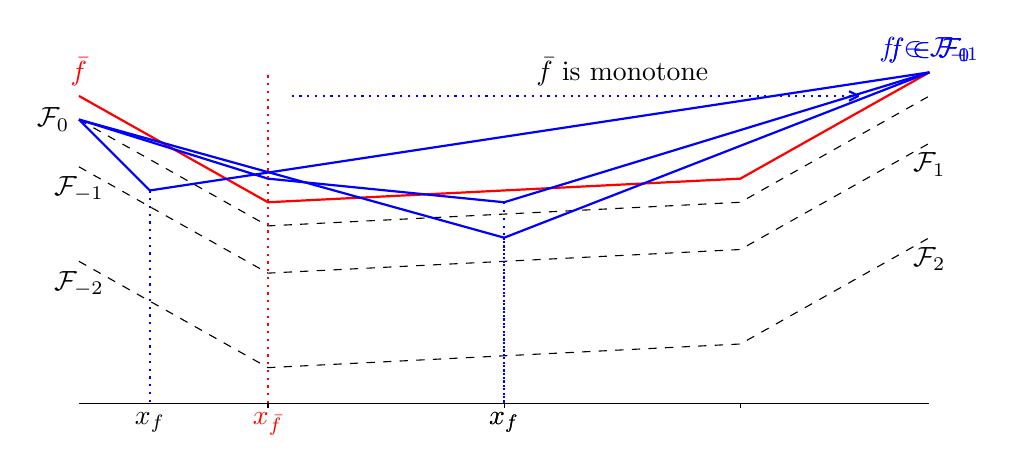
\begin{tikzpicture}[scale=3]
            % bar f
            \draw[thick, red] (-1.8, 1.3) -- (-1,0.85) --(1,0.95) -- (1.8,1.4);
            \node[anchor=south] at (-1.8,1.3) {\textcolor{red}{$\bar f$}};

            %\cF_0
            \uncover<1->{
                \draw[dashed] (-1.8, 1.2) -- (-1,0.75) -- (1,0.85) -- (1.8,1.3);
                \node[anchor=east] at (-1.8,1.2) {$\cF_0$};}

            %f_0
            \uncover<2-2>{
                \draw[thick, blue] (-1.8, 1.2) -- (-1,0.95) --(0,0.85) -- (1.8,1.4);
                \node[anchor=south] at (1.8,1.4) {\textcolor{blue}{$f\in \cF_0$}};
                \draw[thick, blue, dotted] (0,0.85) -- (0,0);
                \node[anchor=north] at (0,0) {$x_f$};
            }

            \uncover<3->{
                \draw[dashed] (-1.8, 1) -- (-1,0.55) -- (1,0.65) -- (1.8,1.1);
                \node[anchor=north] at (-1.8,1) {$\cF_{-1}$};
                \node[anchor=north] at (1.8,1.1) {$\cF_{1}$};
            }

            %vertical
            \uncover<4->{
                \node[anchor=north] at (-1, 0) {\textcolor{red}{$x_{\bar{f}}$}};
                \draw[thick, dotted, red] (-1, 0) -- (-1,1.4);}

            %f_1
            \uncover<5-5>{
                \draw[thick, blue] (-1.8, 1.2) -- (0,0.7) -- (1.8,1.4);
                \node[anchor=south] at (1.8,1.4) {\textcolor{blue}{$f\in \cF_1$}};
                \draw[thick, blue, dotted] (0,0.7) -- (0,0);
                \node[anchor=north] at (0,0) {$x_f$};
            }

            %f_{-1}
            \uncover<6-6>{
                \draw[thick, blue] (-1.8, 1.2) -- (-1.5,0.9) -- (1.8,1.4);
                \node[anchor=south] at (1.8,1.4) {\textcolor{blue}{$f\in \cF_{-1}$}};
                \draw[thick, blue, dotted] (-1.5,0.9) -- (-1.5,0);
                \node[anchor=north] at (-1.5,0) {$x_f$};
            }

            \uncover<7->{
                \draw[dashed] (-1.8, 0.6) -- (-1,0.15) -- (1,0.25) -- (1.8,.7);
                \node[anchor=north] at (-1.8,0.6) {$\cF_{-2}$};
                \node[anchor=north] at (1.8,0.7) {$\cF_{2}$};
            }

            \uncover<8->{
                \draw[blue, thick, dotted] (-0.9,1.3) -> (1.5,1.3);
                \draw[blue, thick] (1.46,1.32) -> (1.5,1.3);
                \draw[blue, thick] (1.46,1.28) -> (1.5,1.3);
                \node[anchor=south] at (0.5, 1.3) {$\bar{f}$ is monotone};
            }

            %axis
            \draw (-1.8,0) -- (1.8,0);
            \draw (0,0) -- (0,-0.02);
            \draw (1,0) -- (1,-0.02);
            \draw (-1,-0) -- (-1,-0.02);

        \end{tikzpicture}
    \end{figure}
\end{frame}


%%%%%%%%%%%%%%%%%%%%%%%%%%%%%%%%%%%%%%%%%%%%%%%%%%%%

\begin{frame}{Upper bounds -- IR bound in 1-D}
    \small
    \textbf{Back to the proof}
    \begin{align*}
        \cF_i & = \begin{cases}
                      \uncover<1->{\{f: \bar f(x_f) - f(x_f) \leq \alpha \}                                                  & \text{if } i = 0}          \\
                      \uncover<3->{\{f: \bar f(x_f) - f(x_f) \in (\alpha 2^{|i|-1}, \alpha 2^{|i|}],\, x_f \geq x_{\bar f}\} & \text{if } i > 0}          \\
                      \uncover<3->{\{f: \bar f(x_f) - f(x_f) \in (\alpha 2^{|i|-1}, \alpha 2^{|i|}],\, x_f < x_{\bar f}\}    & \text{if } i < 0      \,,}
                  \end{cases}
    \end{align*}
    ... and the proof is done through Prop 5 if we show
    \begin{align*}
        \epsilon_i
        \leq
        \alpha + \sqrt{230\inf_{f_1,f_2, f_3,f_4 \in \cF_i} \sum_{j,l \in \pair(4)} (f_j(x_{f_l}) - \bar f(x_{f_l}))^2} \,,
    \end{align*}
    for all $i$ show that with $\epsilon_i = \alpha2^{|i|}$.

    \uncover<2-3>
    {
        \uncover<2-2>{
            \begin{center}
                \textbf{Which trivially holds for $i=0$ since $\epsilon_0 = \alpha$.}
            \end{center}
        }
        \uncover<3->
        {
            \begin{center}
                \textbf{For $i\neq0$ we can use the monotonicity of $\bar{f}$.}
            \end{center}
        }
    }
\end{frame}

%%%%%%%%%%%%%%%%%%%%%%%%%%%%%%%%%%%%%%%%%%%%%%%%%%%%

\begin{frame}{Upper bounds -- IR bound in 1-D}
    \small
    \textbf{Back to the proof for $i \neq 0$ $( \Rightarrow $ monotone $\bar{f}$)}

    % For $i\neq0$ we can use the monotonicity of $\bar{f}$.
    \begin{itemize}
        \item Only 4 functions are enough to get non-negligible disparity.
        \item The proof follows by contradiction.
              Suppose that $x_1 \leq x_2 \leq x_3 \leq x_4$ and
              \begin{align*}
                  \sum_{j,l \in \pair(4)} (f_j(x_{f_l}) - \bar f(x_{f_l}))^2 < c^2 \epsilon^2 \quad \text{for some }c\,,
              \end{align*}
              which means that all $f_1,f_2,f_3,f_4$ are $\epsilon$ close to $\bar{f}$ at all the points $x_1, x_2, x_3, x_4$.
        \item This has to happen while $\bar{f}(x_j) - f_j(x_j) \leq \epsilon_i$ for all $j\in[4]$.
        \item The convexity of $f_1,f_2,f_3,f_4$ and the convexity+monotonicity of $\bar{f}$ in $[x_1, x_4]$ gives the contradiction.
    \end{itemize}
\end{frame}

%%%%%%%%%%%%%%%%%%%%%%%%%%%%%%%%%%%%%%%%%%%%%%%%%%%%

\begin{frame}{Upper bounds -- IR bound in d-D}
    \begin{tcolorbox}[title=Theorem 7 -- IR bound in d-D,colback=blue!5!white,colframe=blue!50!black]
        $(\alpha, \beta \ceil{\log(1/\alpha)}) \in \IR(\cF_{\pb\pl\pr\pm})$ whenever $\alpha \in (0,1)$ and
        \begin{align*}
            \beta = \Omega\left(d^4 \log\left(\frac{d \diam(K)}{\alpha}\right)^2\right) \,.
        \end{align*}
        with the Big-O hiding only a universal constant.
    \end{tcolorbox}
\end{frame}

%%%%%%%%%%%%%%%%%%%%%%%%%%%%%%%%%%%%%%%%%%%%%%%%%%%%

% \begin{frame}{Upper bounds -- IR bound in 1-D}
%     \small
%     We use our decomposition lemma with
%     \begin{align*}
%         \cF_i & = \begin{cases}
%                       \{f \in \cF_{\pb\pl} : \bar f(x_f) - f(x_f) \leq \alpha \}                                                  & \text{if } i = 0          \\
%                       \{f \in \cF_{\pb\pl} : \bar f(x_f) - f(x_f) \in (\alpha 2^{|i|-1}, \alpha 2^{|i|}],\, x_f \geq x_{\bar f}\} & \text{if } i > 0          \\
%                       \{f \in \cF_{\pb\pl} : \bar f(x_f) - f(x_f) \in (\alpha 2^{|i|-1}, \alpha 2^{|i|}],\, x_f < x_{\bar f}\}    & \text{if } i < 0      \,,
%                   \end{cases}
%     \end{align*}
%     \begin{figure}[h!]
%         \begin{tikzpicture}[scale=3]
%             \draw[thick, red] (-1, 0.4) -- (-0.2,-0.1) -- (0.3,0) -- (1,0.33);
%             \draw[thick] (-1,0.5) -- (-0.4, 0) -- (0.25, -0.2) -- (1,0.24);
%             \node[anchor=west] at (1,.24) {$f$};

%             \node[anchor=east] at (-1,0.4) {\textcolor{red}{$\bar f$}};
%             \draw (-1,-0.45) -- (1,-0.45);
%             \draw (0,-0.45) -- (0,-0.47);
%             \draw (1,-0.45) -- (1,-0.47);
%             \draw (-1,-0.45) -- (-1,-0.47);
%             \node[anchor=north] at (0.25, -0.45) {$x_f$};

%             \draw[dotted] (0.25,-0.45) -- (0.25,-0.2);
%             \draw[dashed, blue] (0.25,-0.2) -- (0.25,-0);
%             \draw[blue, thin] (0.27,-0.1) -> (1,-0.1);
%             \draw[blue, thin] (.98,-0.12) -> (1,-0.1);
%             \draw[blue, thin] (.98,-0.08) -> (1,-0.1);
%             \node[anchor=west] at (1, -0.1) {$\bar{f}(x_f) - f(x_f)$};

%             \draw[dotted] (-0.2,-0.45) -- (-0.2,-0.1);
%             \node[anchor=north] at (-0.2, -0.45) {$x_{\bar f}$};


%             \draw[blue, thin, dashed] (-0.2,0.45) -> (1,0.45);
%             \draw[blue, thin] (0.98,0.47) -> (1,0.45);
%             \draw[blue, thin] (0.98,0.43) -> (1,0.45);
%             \node[anchor=south] at (0.5, 0.45) {right (monotone)};

%         \end{tikzpicture}
%     \end{figure}
% \end{frame}

%%%%%%%%%%%%%%%%%%%%%%%%%%%%%%%%%%%%%%%%%%%%%%%%%%%%

% \begin{frame}{Upper bounds -- IR bound in 1-D}
%     \small
%     We use our decomposition lemma with
%     \begin{align*}
%         \cF_i & = \begin{cases}
%                       \uncover<1->{\{f \in \cF_{\pb\pl} : \bar f(x_f) - f(x_f) \leq \alpha \}                                                  & \text{if } i = 0}          \\
%                       \uncover<2->{\{f \in \cF_{\pb\pl} : \bar f(x_f) - f(x_f) \in (\alpha 2^{|i|-1}, \alpha 2^{|i|}],\, x_f \geq x_{\bar f}\} & \text{if } i > 0}          \\
%                       \uncover<2->{\{f \in \cF_{\pb\pl} : \bar f(x_f) - f(x_f) \in (\alpha 2^{|i|-1}, \alpha 2^{|i|}],\, x_f < x_{\bar f}\}    & \text{if } i < 0      \,,}
%                   \end{cases}
%     \end{align*}
%     \only<1-1>{
%         \begin{figure}[h!]
%             \begin{tikzpicture}[scale=3]
%                 % bar f
%                 \draw[thick, red] (-1, 0.4) -- (-0.2,-0.1) -- (0.3,0) -- (1,0.33);
%                 \node[anchor=east] at (-1,0.4) {\textcolor{red}{$\bar f$}};
%                 \draw[dotted] (-0.2,-0.45) -- (-0.2,-0.1);
%                 \node[anchor=north] at (-0.2, -0.45) {$x_{\bar f}$};

%                 % f
%                 \draw[thick] (-1,0.5) -- (-0.4, 0) -- (0.25, 0.05) -- (1,0.24);
%                 \node[anchor=west] at (1,.24) {$f$};
%                 \draw[dotted] (0.25,-0.45) -- (0.25,0.05);
%                 \node[anchor=north] at (0.25, -0.45) {$x_f$};

%                 %axis
%                 \draw (-1,-0.45) -- (1,-0.45);
%                 \draw (0,-0.45) -- (0,-0.47);
%                 \draw (1,-0.45) -- (1,-0.47);
%                 \draw (-1,-0.45) -- (-1,-0.47);

%                 % \draw[dashed, blue] (0.25,-0.2) -- (0.25,-0);
%                 % \draw[blue, thin] (0.27,-0.1) -> (1,-0.1);
%                 % \draw[blue, thin] (.98,-0.12) -> (1,-0.1);
%                 % \draw[blue, thin] (.98,-0.08) -> (1,-0.1);
%                 % \node[anchor=west] at (1, -0.1) {$\bar{f}(x_f) - f(x_f)$};



%                 % \draw[blue, thin, dashed] (-0.2,0.45) -> (1,0.45);
%                 % \draw[blue, thin] (0.98,0.47) -> (1,0.45);
%                 % \draw[blue, thin] (0.98,0.43) -> (1,0.45);
%                 % \node[anchor=south] at (0.5, 0.45) {right (monotone)};

%             \end{tikzpicture}
%         \end{figure}
%         \begin{align*}
%             \epsilon_i  \leq \alpha + \sqrt{230\inf_{f_1,f_2, f_3,f_4 \in \cF_i} \sum_{j,l \in \pair(4)} (f_j(x_{f_l}) - \bar f(x_{f_l}))^2}
%         \end{align*}
%     }
% \end{frame}

%%%%%%%%%%%%%%%%%%%%%%%%%%%%%%%%%%%%%%%%%%%%%%%%%%%%

% \begin{frame}{Upper bounds -- IR bound in 1-D}
%     \small
%     \begin{tcolorbox}[title=Theorem 6 -- IR in 1-D,colback=blue!5!white,colframe=blue!50!black]
%         When $d = 1$, $\sup_{\xi \in \cP(\cF_{\pb\pl})} \BReg_n(\ts, \xi) = O\left(\sqrt{n \log(n) \log(n \diam(\cK))}\right)$.
%     \end{tcolorbox}
%     \begin{figure}[h!]
%         \begin{tikzpicture}[scale=3]
%             \draw[thin] (0,0) -- (0.6,0.02) -- (1,0.22);
%             \draw[thick,red] (0,-0.23) -- (1,0.24);
%             \node[anchor=west] at (1,.24) {$f_1$};

%             \node[anchor=east] at (0,0) {$\bar f$};
%             \draw (-1,-0.25) -- (1,-0.25);
%             \draw (0,-0.25) -- (0,-0.27);
%             \draw (1,-0.25) -- (1,-0.27);
%             \node[anchor=north] at (0.6, -0.25) {$x_2$};
%             % \node[anchor=north] at (0.5,-0.45) {\texttt{(ii)}};
%         \end{tikzpicture}
%         \caption{
%             \texttt{(ii)} shows what happens if $f_3(x_3)$ is too far below $\bar f(x_1)$, which is that $f_3(x_1)$ must be much larger than $\bar f(x_1)$.
%         }
%     \end{figure}
% \end{frame}

%%%%%%%%%%%%%%%%%%%%%%%%%%%%%%%%%%%%%%%%%%%%%%%%%%%%
\begin{frame}{When TS Fails (High-D General Convex)}
    \begin{tcolorbox}[title=Lower Bound 1, colback=red!5, colframe=red!60!black]
        There is a prior on bounded Lipschitz convex functions such that
        \[
            \BReg_T(\text{TS}) \;\ge\; \tfrac12\min\!\bigl\{T,\;e^{\Omega(d)}\bigr\}.
        \]
    \end{tcolorbox}

    \smallskip
    \begin{itemize}
        \item Construction: hide a sharp “valley’’ in a random direction.
        \item TS keeps sampling valleys it hasn’t discovered → linear regret until exponential time.
    \end{itemize}
\end{frame}

%%%%%%%%%%%%%%%%%%%%%%%%%%%%%%%%%%%%%%%%%%%%%%%%%%%%
\begin{frame}{Information-Ratio Barrier}
    \begin{tcolorbox}[title=Lower Bound 2, colback=red!5, colframe=red!60!black]
        For general convex losses the classical info-ratio machinery cannot give regret
        better than \(\widetilde{O}(d^{1.5}\sqrt{T})\).
    \end{tcolorbox}

    \begin{itemize}
        \item Matches best known algorithmic upper bound.
        \item Suggests new ideas needed for \( \widetilde{O}(d\sqrt{T}) \) in adversarial BCO.
    \end{itemize}
\end{frame}

%%%%%%%%%%%%%%%%%%%%%%%%%%%%%%%%%%%%%%%%%%%%%%%%%%%%
\begin{frame}{Conclusion}
    \begin{itemize}
        \item Thompson sampling Bayesian upper bound for 1-D convex bandits.
        \item Structured high-D (monotone ridge) \(\Rightarrow\) $\tilde{O}(d^{2.5}\sqrt{n})$ regret.
        \item TS suffers \emph{exponential in $d$} for general convex losses in $\R^d$.
        \item Classic IR analysis can't be used to beat the $O(d^{1.5}\sqrt{n})$ upper bound for adversarial BCO.
    \end{itemize}

    \bigskip
    \centering
    \textbf{Thanks!}\\
    \smallskip
\end{frame}

%%%%%%%%%%%%%%%%%%%%%%%%%%%%%%%%%%%%%%%%%%%%%%%%%%%%
\end{document}